\documentclass[11pt]{article}
\usepackage[margin=1in]{geometry}

\usepackage{amsmath}
\usepackage{amssymb}
\usepackage{physics}
\usepackage{graphicx}

\usepackage{hyperref}

\renewcommand{\d}[2][]{\mathrm{d}^{#1}{#2}}



\begin{document}


\section{Introduction}


\begin{itemize}
    \item 1605.01735, \textit{Machine Learning Phases of Matter}, Carrasquilla \& Melko: Used supervised learning with neural-network to classify raw spin configurations into two phases for classical Ising model, square-ice model and gauged Ising model. The trained network for the square-lattice classical Ising model correctly identifies the critical temperature for triangular-lattice classical Ising model without ``information about the Hamiltonian, the lattice structure, or even the general locality of interactions". For the square-ice and gauged Ising models where there is no conventional order parameter, the are able to distinguish between the ground and high-temperature states.
    \item 1606.00318, \textit{Discovering Phase Transitions with Machine Learning}, Lei Wang: Used the unsupervised methods of PCA and clustering to identify phase transitions and order parameters using raw spin configurations in classical Ising model and COP Ising model ($\sum\sigma=0$).
    \item 1609.02552, \textit{Machine Learning Phases of Strongly Correlated Fermions}, Ch'ng et.al.: Used neural-network to identify phases in 3d Hubbard model of fermions on cubical lattice.
    \item 1610.02048, \textit{Learning Phases of Matter by Confusion}, van Nieuwenburg et.al.: Unsupervised methods of PCA and clustering on the entanglement spectrum or Kitaev model clearly identifies different topological phases. Supervised learning with neural-network identifies phases as well, even when omitting a region around the phase-transition point. Their ``confusion scheme" systematically trains on data incorrectly labelled according to a tunable parameter. Asking when the accuracy of the trained network is highest on the entire data set narrows in on the ``correct" value of the parameter and thus the location of the phase transition. This scheme is applied to the classical Ising model in 2d and the random-field Heisenberg chain.
    \item 1703.02435, \textit{Unsupervised learning of phase transitions: from principal component analysis to variational autoencoders}, Wetzel: Used unsupervised methods of PCA and variational autoencoder on 2d classical Ising model and 3d XY model.
    \item 1704.00080, \textit{Discovering Phases, Phase Transitions and Crossovers through Unsupervised Machine Learning: A critical examination}, Hu et.al.: Used PCA and autoencoders to identify phase transitions in square and triangular Ising models, biquadratic-exchange spin-one Ising model (highly degenerate). Blume-Capel model (both first- and second-order transitions) and 2d XY model.
\end{itemize}

Some methods:
\begin{itemize}
    \item PCA: dimensionally reduce data to hyperplane where variance is largest (principal axes).
    \item Autoencoder: ``dimensional reduction" idea applied to neural-networks. Have a hidden layer with very few nodes and train the network to reconstruct data similar to input data based just on that hidden layer (put a bottle-neck in neural network).
\end{itemize}


\section{TDA}
For any discrete data set, persistent homology entails a sequence of simplicial complexes ($\alpha$, Vietoris-Rips, \&c.) of varying granularity in which homological cycles first appear and then disappear. The choice in filtration corresponds to different ways to add edges and faces to the simplicial complex as some parameter is varied. This process produces a collection of persistence data consisting of births and deaths, $\{b_i,d_i\}$, for each of the cycles. Persistence diagrams are a way to visualize these topolgically derived data.

The persistence diagram contains information about the size of features in the data. Since such topological data are robust against small perturbations in the original data set, TDA is a useful tool in statistical analyses of many systems.


(Why persistence image is necessary... robustness against sudden appearence of cycles, small perturbations in persistence data, \&c.) To create the persistence image, begin by transforming the persistence data to $\{b_i,p_i\}=\{b_i,d_i-b_i\}$. Each point is then smoothed, which allows for small perturbations in the topological data to have small effects. Choosing gaussians of fixed width, the full density is
\begin{align}
    \rho(x,y) &= \sum_i w(b_i,p_i)\;\frac{1}{2\pi\sigma^2}\exp\left[-\frac{(x-b_i)^2+(y-p_i)^2}{2\sigma^2}\right]
\end{align}
The weighting function should be chosen so that $w(b_i,0)=0$; this ensures that the sudden appearence of a cycle is accounted for smoothly. For simplicity, we choose $w(b_i,p_i)=p_i$. Because of the lattice structure for these spin models the set of possible $(b_i,p_i)$ pairs is discrete, and we find it convenient to compute $\rho$ as
\begin{align}
    \rho(x,y) &= \sum_{(b,p)}N_{b,p}\times w(b,p)\;\frac{1}{2\pi\sigma^2}\exp\left[-\frac{(x-b)^2+(y-p)^2}{2\sigma^2}\right]
\end{align}
for $N_{b,p}$ the frequency of the $(b,p)$ pair. As for choosing $\sigma$, we have a natural length-scale which is the lattice size. Can compare varying choice of $\sigma$.


The persistence image is then the vector obtained by integrating $\rho$ over a series of ``pixels'' (bins):
\begin{align}
    I_\text{p} &= \iint\limits_\text{p}\rho(x,y)\,\d{x}\d{y}
\end{align}
This process can be done for $H_0,H_1,\ldots$ and the respective vectors adjoined or treated separately. Ultimately, we have now a vector in $\mathbb{R}^n$ ($n$ not too large!) which is a representation of the homological structure of the original data set.

\begin{figure}[t]
    \centering
    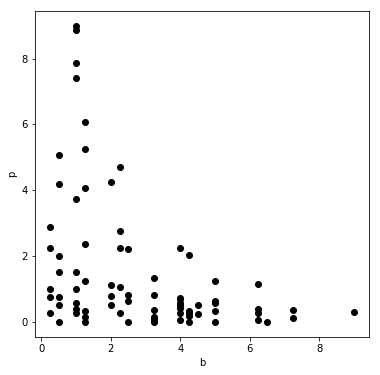
\includegraphics[width=0.3\textwidth]{pd_example}
    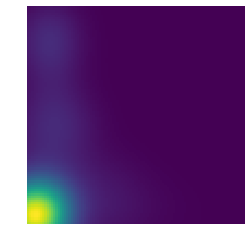
\includegraphics[width=0.3\textwidth]{rho_example}
    
\includegraphics[width=0.3\textwidth]{pi_example}
    \caption{Example PD$\rightarrow\rho\rightarrow$PI process. Because of the lattice structure many points in the persistence diagram coincide.}
\end{figure}

(The above should be altered slightly for $H_0$ since in this case the persistence data are essentially one-dimensional.)


\section{Spin Models}
Here we will apply the techniques of TDA to lattice spin systems. The traditional Ising model is rich in behaviour, despite being simple to describe; in two or more dimensions there is a second-order phase transition from an ordered to random state. While it is relatively easy to distinguish between these states simply by looking at the spin configurations, there exist systems in which the different states are not as readily identified. It has been demonstrated that one can use machine learning to identify phases of matter for such spin systems. We will show that this classification can also be done using persistance images built from the spin configurations, where physical characteristics of the data such as sizes of features play a central role.

We take as data the physical locations of spins which all point in the same direction as the majority of spins after reaching equilibrium with a thermal bath. To generate sample spin configurations, we use Monte Carlo methods, characterized by the following:
\begin{itemize}
    \item $N$: Linear size of periodic lattice. May not correspond to number of spins, e.g.~if spins are not on vertices but on edges.
    \item $\{T_i\}$: Collection of temperatures used.
    \item $N_\text{sim}$: Number of simulations at each temperature.
    \item $K$: Measure of the number of Monte Carlo iterations, being the average number of flips per spin.
\end{itemize}
For each simulation we create a persistence image, which depends on the following choices:
\begin{itemize}
    \item $w(b,p)$: Weighting factor to emphasize longer-lived features. Stability requires $w(b,0)=0$. We choose $w(b,p)=p$ for simplicity.
    \item $\sigma$: Size of gaussians for smoothing process. We have a natural length-scale in our set-up, which is the lattice spacing ($l=1$). Have been using $\sigma=1$, but a comparison for different $\sigma$ would be good to have.
    \item $\{\text{p}_i\}$: Collection of pixels/bins to be integrated over to yield the persistence images. Have been using $1\times 1$ pixels.
\end{itemize}
After having created these persistence images we have the following methods for identifying phases and critical temperatures:
\begin{itemize}
    \item Logistic regression (supervised learning, identify phase): With a known critical temperature, can train on a subset of the persistence images labelled by their phase. When applied to testing data can quantify accuracy of the regression by comparing to known phase designations.
    \item $k$-means clustering (unsupervised learning, identify phase): Train on a subset of the persistence images, learning appropriate locations for cluster ceneters. When applied to testing data of known temperature can ask what percentage are placed in one cluster or the other, with the critical temperature being where this crosses 50\%. The accuracy at each temperature can also be quantified, since the ``correct'' cluster is known.
    \item PCA (data visualization): Project the high-dimensional persistence images onto the plane for which the variance is largest.
\end{itemize}

The models we choose are increasing non-local. We begin with the classical Ising model, which is exactly solved for $d=2$ and very well-studied for $d=3$. This is the easiest to classify into two phases based on the spontaneous magnetization below the critical temperature. Next is the square-ice (a.k.a.~16 vertex) model, which has no spontaneous magnetization but rather a transition from power-law to exponentially decaying spin-spin correlation functions. Finally, the $\mathbb{Z}_2$-gauged Ising model has a local gauge symmetry which implies no spontaneous magnetization and requiresgauge-invariant to be gauge-invariant in order that they be well-defined. By considering correlation functions aroung loops in the lattice, one finds a phase transition from ``perimeter'' to ``area'' law for $d\geq 3$: there is no phase transition for $d=2$.

\newpage
\subsection{Classical Ising Model}
For the classical Ising model in $d$ dimensions one uses the cubical lattice $\mathbb{Z}_N^d$ with spins located at the vertices taking values in $\{{-1},1\}$. Interactions are local, being between pairs of adjacent spins. The Hamiltonian is
\begin{equation}
    H = -\sum_{\langle i,j\rangle}s_is_j
\end{equation}
where $\langle i,j\rangle$ denotes all nearest-neighbor pairs. We work with a finite lattice of $N^d$ spins and periodic boundary conditions. At $T=0$ the energy per spin is $-d$ and at $T=\infty$ the energy per spin is zero.

The Ising model has a second-order phase transition for all $d\geq 2$, characterized by a spontaneous magnetization at low temperatures. In the thermodynamic limit, $N\to\infty$, the critical temperatures in 2d and 3d are $T_\text{c}\approx 2.269$ and $T_\text{c}\approx4.512$, respectively. With finite $N$ we expect the critical temperatures to be shifted slightly to larger values.

Away from the critical point spin-spin correlation functions decay exponentially, but at the critical point they follow a power-law ($\ev{s_0s_r}\sim r^{-1/4}$ in 2d and $\ev{s_0s_r}\sim r^{-1.036}$ in 3d), i.e.~the correlation length diverges. TO DO: can these critical exponents be extracted from the persitence diagrams/images?

To sample configurations weighted by the Boltzmann factor $e^{-\beta H}$ we use the Wolff cluster algorithm with the following parameters:
\begin{align}
    2d&\sim\left\{\begin{array}{l}
        N = 50\\
        \{T_i\} = \{1.00,1.05,\ldots,3.50\}\\
        N_\text{sim} \approx 1400 (?)\\
        K = 20
    \end{array}\right. & 3d&\sim\left\{\begin{array}{l}
        N = 15\\
        \{T_i\} = \{3.00,3.05,\ldots,6.00\}\\
        N_\text{sim} = 1000 (?)\\
        K = 20
    \end{array}\right.
\end{align}
Examples of low- and high-temperature spin configurations are shown in figure~\ref{fig:IsingExampleConfigs}. Since the persistence diagrams often extend to $b,p\sim 25$ we use $1\times 1$ pixels extending out to $b=25$ and $p=25$ (persistence images are elements of $\mathbb{R}^{625}$).

\begin{figure}[h]
    \centering
    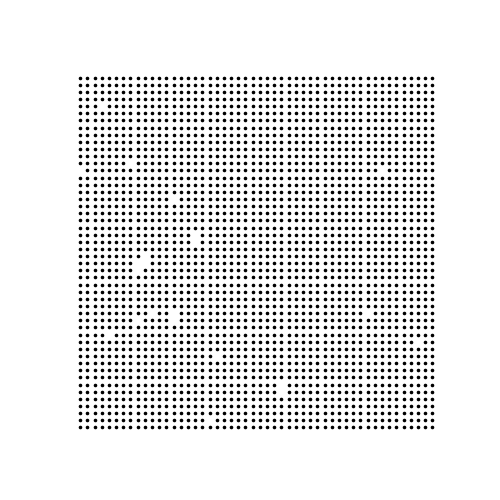
\includegraphics[width=0.3\textwidth]{ising_images/ising_T=150.png}
    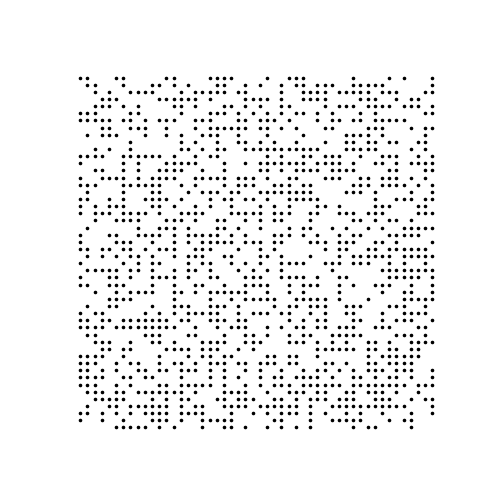
\includegraphics[width=0.3\textwidth]{ising_images/ising_T=inf.png}
    \caption{Example configurations for 2d Ising model at $T=1.5$ (left) and $T=\infty$ (right).}
    \label{fig:IsingExampleConfigs}
\end{figure}

\newpage
\subsubsection{$k$-Means}
Here the clustering algorithm separates the training persistence images into two clusters. For $d=2$ the critical temperature is estimated as $T_\text{c}\approx 2.3246$ (see figure~\ref{ref:IsingKmeans}). This is within 2.5\% of the exact value of $T_\text{c}$ in the thermodynamic limit, a discrepancy which is easily attributed to finite-$N$ effects.

\begin{figure}[h]
    \centering
    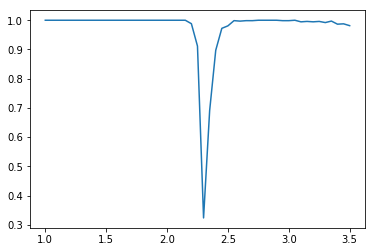
\includegraphics[width=0.3\textwidth]{ising_images/kmeans_2d_ising}
    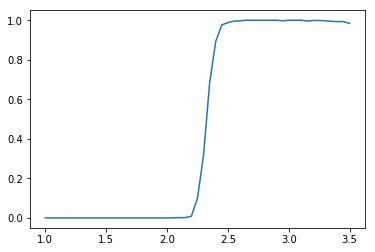
\includegraphics[width=0.3\textwidth]{ising_images/kmeans_avg_2d_ising}
    \caption{Left: accuracy on testing data. Right: average classification on testing data. The cross-over point gives an estimate for the critical temperature, $T_\text{c}\approx 2.3246$.}
    \label{ref:IsingKmeans}
\end{figure}


\subsubsection{Logistic Regression}
For $d=2$ we label persistence images to be in the ordered phase for $T<2.269$. The logistic regression depends heavily on small, short-lived cycles to distinguish between the ordered and disordered phases (see left of figure~\ref{fig:IsingLogReg}). Accuracy is near 100\% for most temperatures, and the cross-over point occurs at $T\approx 2.2796$.

\begin{figure}[h]
    \centering
    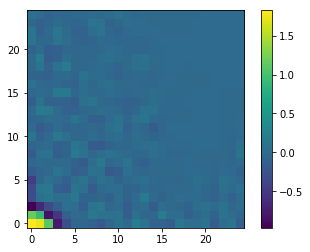
\includegraphics[width=0.24\textwidth]{ising_images/logreg_2d_ising}
    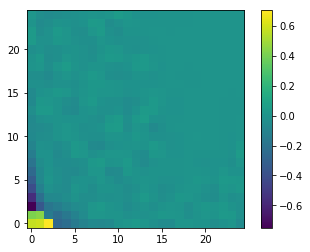
\includegraphics[width=0.24\textwidth]{ising_images/logreg2_2d_ising}
    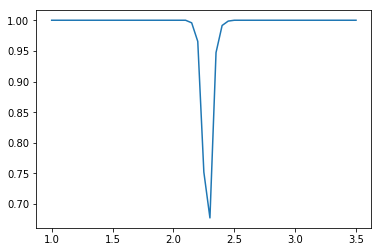
\includegraphics[width=0.24\textwidth]{ising_images/logreg_acc_2d_ising}
    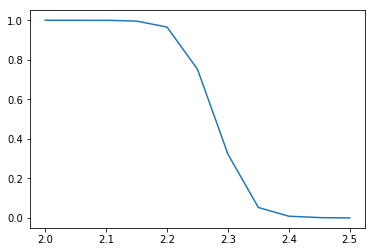
\includegraphics[width=0.24\textwidth]{ising_images/logreg_avg_2d_ising}
    \caption{Left: coefficients for logistic regression with $C=0.1$ and $L_2$ penalty. Left center: coefficients for logistic regression with $C=0.01$ and $L_2$ penalty. Right center: accuracy on testing data. Right: average classification on testing data. The cross-over point gives an estimate for the critical temperature, $T_\text{c}\approx 2.2796$.}
    \label{fig:IsingLogReg}
\end{figure}

There are few surprises here - the spontaneous magnetization allows for an easy classification based on the number of small islands of minority spins. In fact one could do a logistic regression on the raw spin configurations and achieve the same result, as it can effectively reconstruct the order parameter, $m=\ev{|\sum s_i|}$.

\subsubsection{PCA}
PCA for $d=2$ leads to a clear trend in temperature (judging from other work, diagram would be symmetric if we chose majority/minority spins randomly).

\begin{figure}[h]
    \centering
    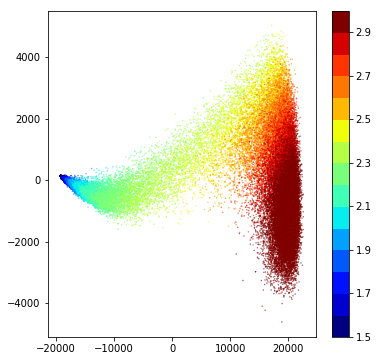
\includegraphics[width=0.24\textwidth]{ising_images/pca_2d_ising}
    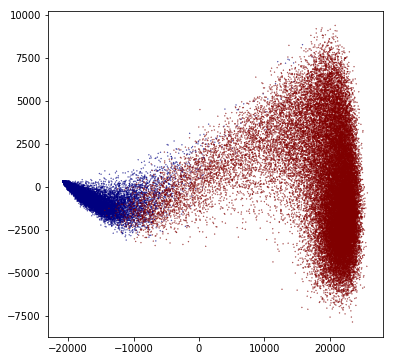
\includegraphics[width=0.24\textwidth]{ising_images/pca_phase_2d_ising}
    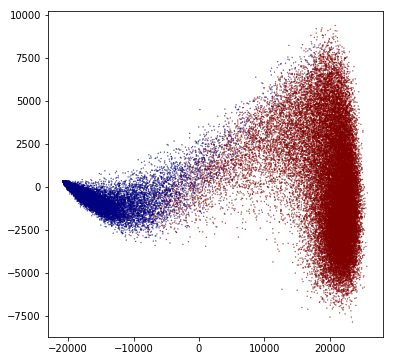
\includegraphics[width=0.24\textwidth]{ising_images/pca_phase2_2d_ising}
    \caption{Left: PCA colored by temperature. Center: PCA colored by phase, taking $T_\text{c}=2.269$. Right: PCA colored by phase, taking $T_\text{c}=2.3246$}
    \label{fig:IsingPCA}
\end{figure}


\subsection{Square Ice Model}
We consider the square ice model on the cubical lattice $\mathbb{Z}_N^d$ with spins located on edges between adjacent vertices taking values in $\{{-1},1\}$. The Hamiltonian is
\begin{equation}
    H = \sum_v\Big(\sum_{i\in v}s_i\Big)^2
\end{equation}
where $v\in\mathbb{Z}_N^d$ and by $i\in v$ we mean those edges connecting to the vertex $v$. We work with a finite lattice of $dN^d$ spins and periodic boundary conditions. At $T=0$ the energy per spin is zero and at $T=\infty$ the energy per spin is two.

This model has a (?-order) phase transition for all $d\geq 2$ as the spin-spin correlation functions go from being power-law at low temperatures to exponentially decaying at high temperatures.

To sample configurations weighted by the Boltzmann factor $e^{-\beta H}$ we use a Monte Carlo algorithm with the following parameters:
\begin{align}
    2d&\sim\left\{\begin{array}{l}
        N = 50\\
        \{T_i\} = \{0.0,0.1,\ldots,4.0\}\\
        N_\text{sim} = 1000(?)\\
        K = 200
    \end{array}\right. & 3d&\sim\left\{\begin{array}{l}
        N = 15\\
        \{T_i\} = \{0.0,0.1,\ldots,4.0\}\\
        N_\text{sim} = 1000(?)\\
        K = 200
    \end{array}\right.
\end{align}
Examples of low- and high-temperature spin configurations are shown in figure~\ref{fig:SquareiceExampleConfigs}. Since the persistence diagrams are very concentrated near the origin, we use $0.5\times0.5$ pixels extending out to $b=5$ and $p=5$ (persistence images are elements of $\mathbb{R}^{100}$).

\begin{figure}[h]
    \centering
    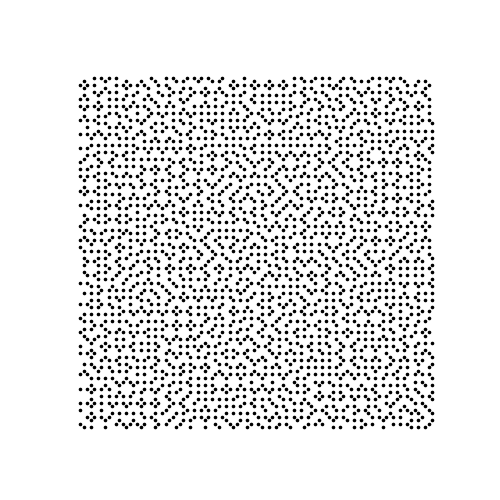
\includegraphics[width=0.28\textwidth]{squareice_images/squareice_T=0.png}
    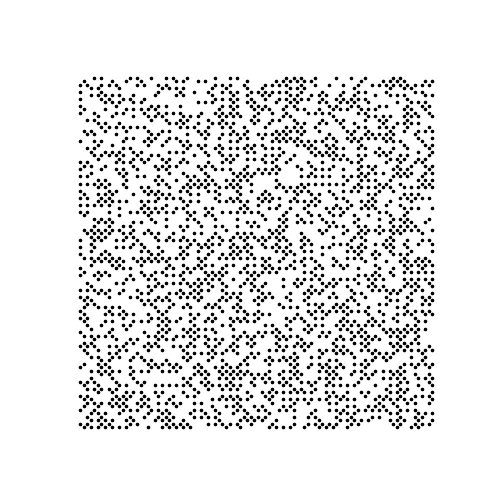
\includegraphics[width=0.28\textwidth]{squareice_images/squareice_T=inf.png}
    \caption{Example configurations for square ice model at $T=0$ (left) and $T=\infty$ (right).}
    \label{fig:SquareiceExampleConfigs}
\end{figure}

\newpage
\subsubsection{$k$-Means}

\begin{figure}[h]
	\centering
	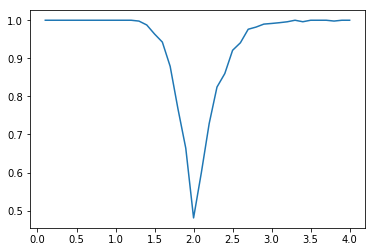
\includegraphics[width=0.3\textwidth]{squareice_images/kmeans_2d_squareice}
	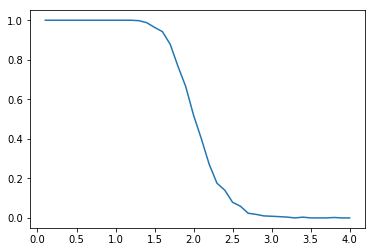
\includegraphics[width=0.3\textwidth]{squareice_images/kmeans_avg_2d_squareice}
	\caption{Left: accuracy on testing data. Right: average classification on testing data. The cross-over point gives an estimate for the critical temperature, $T_\text{c}\approx 2.0166$.}
\end{figure}


\subsubsection{Logistic Regression}
Labelling persistence images using the critical temperature found by $k$-means clustering, can train logistic regression.

\begin{figure}[h]
    \centering
    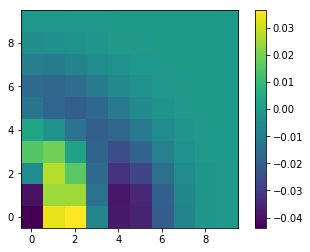
\includegraphics[width=0.3\textwidth]{squareice_images/logreg_2d_squareice}
    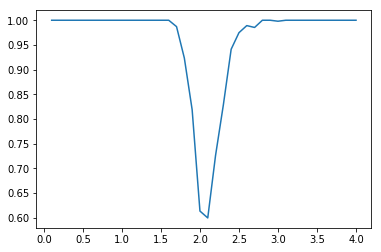
\includegraphics[width=0.3\textwidth]{squareice_images/logreg_acc_2d_squareice}
    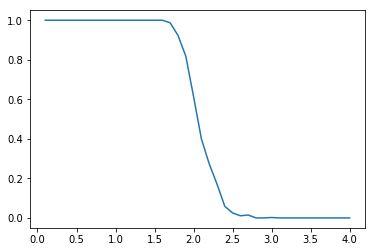
\includegraphics[width=0.3\textwidth]{squareice_images/logreg_avg_2d_squareice}
    \caption{Left: coefficients for logistic regression with $C=0.1$ and $L_2$ penalty. Center: accuracy on testing data. Right: average classification on testing data. The cross-over point gives an estimate for the critical temperature, $T_\text{c}\approx 2.0527$.}
    \label{fig:SquareiceLogReg}
\end{figure}


\subsubsection{PCA}
For $d=2$ we have a clear trend in temperature and the projection of the $k$-means clusters reveals the two-cluster structure.
\begin{figure}[h]
    \centering
    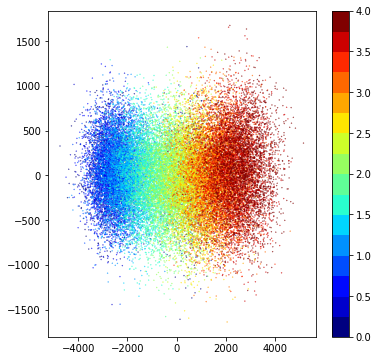
\includegraphics[width=0.25\textwidth]{squareice_images/pca_2d_squareice}
    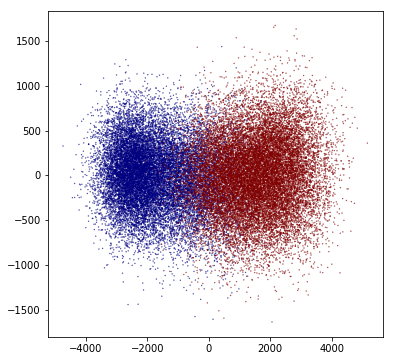
\includegraphics[width=0.26\textwidth]{squareice_images/pca_phase_2d_squareice}
    \caption{Left: PCA colored by temperature. Right: PCA colored by phase, taking $T_\text{c}\approx2.02$.}
    \label{fig:SquareicePCA}
\end{figure}

\newpage
\subsection{$\mathbb{Z}_2$-Gauged Ising Model}
(see [\textit{Gauge fields...}, Balian et.al.])

A variant of the classical Ising model where the global $\mathbb{Z}_2$ symmetry has been promoted to a local (gauge) symmetry is considered as well. The model is defined on the cubical lattice $\mathbb{Z}_N^d$ with spins located on edges between adjacent vertices taking values in $\{{-1},1\}$. The Hamiltonian is
\begin{equation}
    H = - \sum_f\prod_{i\in f}s_i
\end{equation}
where $f$ denote faces, or plaquettes, and by $i\in f$ we mean those four edges consisting of the boundary of $f$. The local $\mathbb{Z}_2$ symmetry corresponds to $H$ being invariant under the flipping of all $2d$ spins on edges connected to any single vertex (this necessarily flips either zero or two spins on each plaquette). We work with a finite lattice of $dN^d$ spins and periodic boundary conditions. At $T=0$ the energy per spin is $\frac{1-d}{2}$ and at $T=\infty$ the energy per spin is zero.

The gauge-invariance guarantees that there is no spontaneous magnetization, and restricting to gauge-invariant observables rules out considering spin-spin correlation functions. An appropriate observable is found by considering a closed path $C$ in the lattice and the expectation value of the product of the spins around this path. In dimensions $d>2$ a phase transition is signalled by a change in such correlation functions: at low temperature one finds a ``perimeter law",
\begin{equation}
    \Big\langle\prod_C s_i\Big\rangle \sim e^{-h(\beta)L} \qquad\qquad h(\beta) = 2e^{-4(d-1)\beta} + \cdots
\end{equation}
while at high temperatures one finds an ``area law",
\begin{equation}
    \Big\langle\prod_C s_i\Big\rangle \sim e^{-f(\beta)A} \qquad\qquad f(\beta) = -\log\operatorname{arctanh}{\beta} + \cdots
\end{equation}
for $L$ the length of the path $C$ and $A$ the minimum number of plaquettes needed to span $C$. The arguments which lead to these expressions do not apply in $d=2$ (see section V.D.~of [\textit{An introduction...}, Kogut]) as the radius of convergence for the validity of the perimeter law is zero. One may also understand the special case of $d=2$ as being a consequence of the equivalence
\begin{equation}
    \big(\text{2d }\mathbb{Z}_2\text{-gauged Ising model}\big) = \big( \text{1d classical Ising model} \big)
\end{equation}
found by comparing the partition functions of the two models after having chosen a convenient gauge. One can, however, still hope to distinguish between high and low temperature spin configurations, as correlation length does change with temperature.

For $d>2$ we can hope to do more: not only identify high and low temperature configuration but also determine the critical temperature at which one shifts from a perimeter to area law.

To sample configurations weighted by the Boltzmann factor $e^{-\beta H}$ we use a Monte Carlo algorithm with the following parameters:
\begin{align}
    2d&\sim\left\{\begin{array}{l}
        N = 50\\
        \{T_i\} = \{0,?\}\\
        N_\text{sim} = 1000(?)\\
        K = 200
    \end{array}\right. & 3d&\sim\left\{\begin{array}{l}
        N = 15\\
        \{T_i\} = \{?\}\\
        N_\text{sim} = 1000(?)\\
        K = 200
    \end{array}\right.
\end{align}
Examples of low- and high-temperature spin configurations are shown in figure~\ref{fig:GaugedExampleConfigs}.

\begin{figure}[h]
    \centering
    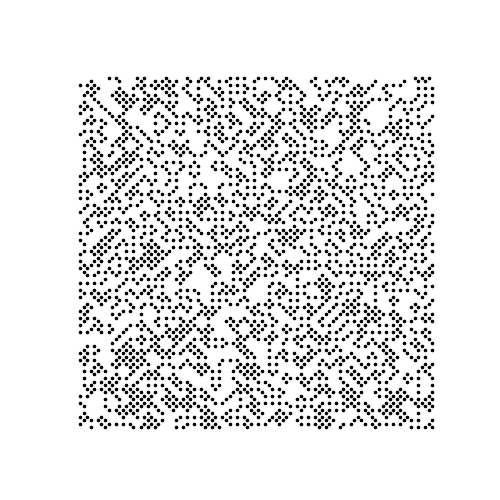
\includegraphics[width=0.3\textwidth]{gauged_images/gauged_T=0.png}
    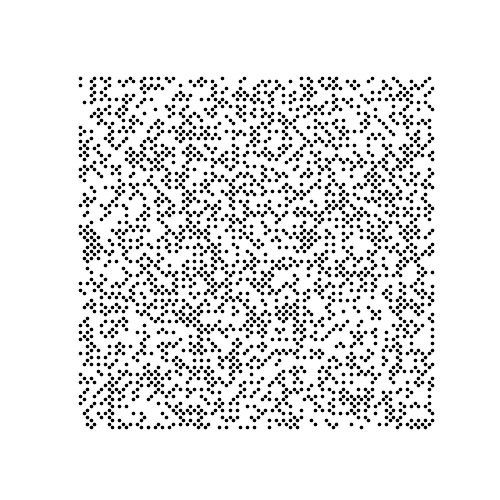
\includegraphics[width=0.3\textwidth]{gauged_images/gauged_T=inf.png}
    \caption{Example configurations for the $\mathbb{Z}_2$-gauged Ising model at $T=0$ (left) and $T=\infty$ (right).}
    \label{fig:GaugedExampleConfigs}
\end{figure}





\end{document}